Author: Joe Corneli

\begin{quote}
The word ``learning'' does not adequately capture what it means to
figure out the ``\emph{for what purpose or reason}'' dimension that is
essential for a peeragogical endeavor. Interpersonal exchange and
collaboration to develop and pursue common goals goes further than
``learning'' or ``working'' in their mainstream definitions. This
article will look at examples drawn from Linux, Wikipedia, and my own
work on PlanetMath, with a few surprises along the way, leading us to
new ways of thinking about how to do co-design when build systems for
peer learning and peer production.
\end{quote}
\subsection{Co-working as the flip side of convening}

\begin{quote}
\textbf{Linus Torvalds}: The first mistake is thinking that you can
throw things out there and ask people to help. That's not how it works.
You make it public, and then you assume that you'll have to do all the
work, and ask people to come up with suggestions of what you should do,
not what they should do. Maybe they'll start helping eventually, but you
should start off with the assumption that you're going to be the one
maintaining it and ready to do all the work. The other thing--and it's
kind of related--that people seem to get wrong is to think that the code
they write is what matters. No, even if you wrote 100\% of the code, and
even if you are the best programmer in the world and will never need any
help with the project at all, the thing that really matters is the users
of the code. The code itself is unimportant; the project is only as
useful as people actually find it.

\end{quote}
In fact, we can think of contributors as a special class of ``user''
with a real time investment in the way the project works. We typically
cannot ``Tom Sawyer'' ourselves into leisure or ease just because we
manage to work collaboratively, or just because we have found people
with some common interests. And yet, in the right setting, many people
do want to contribute! For example, on ``Wikipedia, the encyclopedia
anyone can edit'' (as of 2011)
\href{http://\%20http://www.readwriteweb.com/archives/wikipedias\_goal\_1\_billion\_monthly\_visitors\_by\_2015.php}{as
many as} 80,000 visitors make 5 or more edits per month. 

This is interesting to compare with the
\href{http://www.aaronsw.com/weblog/whowriteswikipedia}{empirical fact}
that (as of 2006) ``over 50\% of all the edits are done by just .7\% of
the users\ldots{} 24 people\ldots{}and in fact the most active 2\%,
which is 1400 people, have done 73.4\% of all the edits.'' Similar
numbers apply to other peer production communities.

\begin{center}
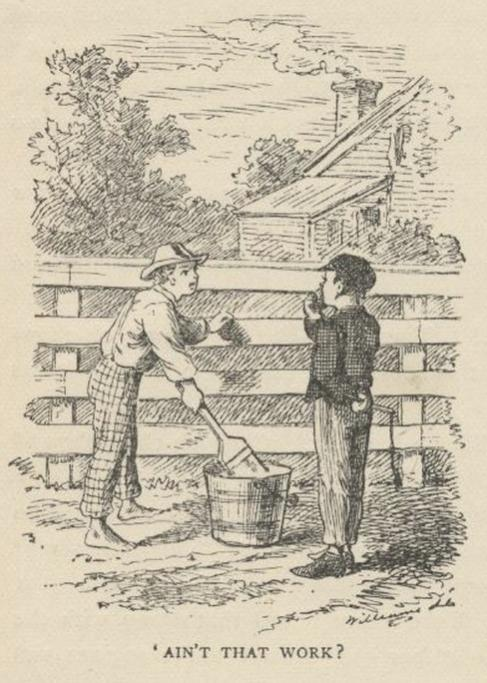
\includegraphics[width=.5\textwidth]{../pictures/tom-sawyer.jpeg}
\end{center}

\subsection{A little theory}

In many natural systems, things are not distributed equally, and it is
not atypical for e.g. 20\% of the population to control 80\% of the
wealth (or, as we saw, for 2\% of the users to do nearly 80\% of the
edits). Many, many systems work like this, so maybe there's a good
reason for it.

Let's think about it in terms of ``coordination'' as understood by the
late Elinor Ostrom. She talked about ``local solutions for local
problems''. By definition, such geographically-based coordination
requires close proximity. What does ``close'' mean? If we think about
homogeneous space, it just means that we draw a circle (or sphere)
around where we are, and the radius of this circle (resp. sphere) is
small. An interesting
\href{http://en.wikipedia.org/wiki/N-sphere\#Volume\_and\_surface\_area}{mathematical
fact} is that as the dimension grows, the volume of the sphere gets
``thinner'', so the radius must increase to capture the same
\emph{d}-dimensional volume when \emph{d} grows! In other words, the
more different factors impact on a given issue, the less likely there
are to be small scale, self-contained, ``local problems'' or ``local
solutions'' in the first place.

As a network or service provider grows (like a
\href{http://peeragogy.org/organize/connectivism-in-practice-how-to-organize-a-mooc/}{MOOC}
as opposed to a
\href{http://peeragogy.org/case-study-collaborative-explorations/}{Collaborative
Exploration}, for example), they typically build many weak ties, with a
few strong ties that hold it all together. Google is happy to serve
everyone's web requests -- but they can't have just anyone walking in
off the street and connecting devices their network in Mountain View. By
the way, the 2006 article on Wikipedia quoted above was written by Aaron
Swartz (``over 50\% of all the edits are done by\ldots{} 24 people'',
etc.), who achieved considerable
\href{http://www.wired.com/threatlevel/2011/07/swartz-arrest/}{notoriety}
for doing something similar with MIT's network. His is a particularly
sad case of one person acting alone and drawing significant ire from
institutions and governments; we could contrast Aaron Swartz, the
individual, with the peer-to-peer infrastructures like the ones that run
PirateBay, which have proved much harder to stop.

\subsection{Co-working: what is an institution?}

As idealists, we would love to be able to create systems that are both
powerful and humane. Some may reflect with a type of sentimental
fondness on completely mythical economic systems in which a ``dedicated
individual could rise to the top through dint of effort.''
Well-articulated systems like this \emph{do} exist, however: natural
languages, for example, are so expressive and adaptive that most
sentences have never been said before. A well-articulated system lends
itself to ``local solutions to local problems'' -- but in the
linguistics case, this is only because all words are not created equal.

\begin{quote}
\textbf{Dr Seuss}: My brothers read a little bit. Little words like `If'
and `It.' My father can read big words, too, Like CONSTANTINOPLE and
TIMBUKTU.
\end{quote}
We could go on here to talk about Coase's theory of the firm, and
Benkler's theory of
"\href{http://www.yale.edu/yalelj/112/BenklerWEB.pdf}{Coase's Penguin}".
We might continue
\href{http://www.aaronsw.com/weblog/perfectinstitutions}{quoting} from
Aaron Swartz. But we will not get so deeply into that here: you can
explore it on your own! For now, it is enough to say that an institution
is a bit like a language. This will help us a lot in the next section.

\subsection{Designing a platform for peer learning\emph{}}

\begin{quote}
\href{planetmath.org}{PlanetMath} is\emph{a virtual community which aims
to help make mathematical knowledge more accessible}.
\end{quote}
In my PhD thesis {[}1{]}, I talk about my work to turn this long-running
website, which since 2001 had focused on building a mathematics
encyclopedia, into a peer produced peer learning environment. The
picture below shows the basic idea. We would retain all of the old
activities related to authoring, reviewing, and discussing encyclopedia
articles, but we would also add a bunch of new features having to do
with mathmatical problem solving, an activity that is suitable for
mathematical beginners.

\begin{center}
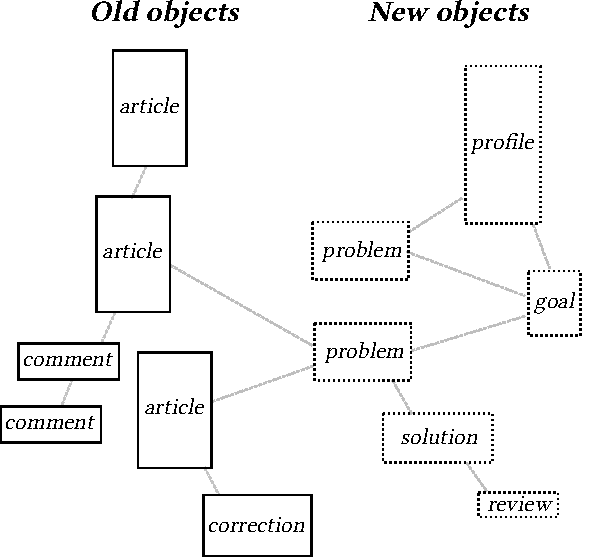
\includegraphics[width=.65\textwidth]{../pictures/extension-to-develop.pdf}
\end{center}

My first translation of that sketch into a basic interaction design was
as follows. People can continue to add articles to PlanetMath's
encyclopedia: they can connect one article to another either by making
one article the ``parent'' of another ($A \leftarrow A\,$), or, more typically, via an inline link $\ell$.  Like in the old system,
users can discuss any object ($X  \leftarrow T\,$),
but now there is more structure: \emph{problems} can be connected to
articles ($A \leftarrow P\,$) and \emph{solutions} can be connected to problems
($P\leftarrow S\,$). Instead of explicitly modeling ``goals,'' the idea I came up with
was that problems and articles could be organized into ``collections,''
the same way that videos are organized into playlists on YouTube, and
that the user would get encouraging feedback as they work their way
through the problems in a given collection. I described a few other
types of objects and interactions that were not present in the above
sketch, like questions and answers, groups, and the ability to change
the ``type'' of certain contributed objects. This table summarizes the
overall design.

\begin{center}
{\Tiny
\begin{tabular}{| >{\centering\arraybackslash}m{.15\textwidth} | >{\centering\arraybackslash}m{.15\textwidth} | >{\centering\arraybackslash}m{.15\textwidth} | >{\centering\arraybackslash}m{.15\textwidth} | >{\centering\arraybackslash}m{.17\textwidth}| }
\hline
Context & Feedback & Quality & Structure & Heuristic \\[.2mm]
\hline
\vspace{.2mm}
$\begin{array}{c}
A \leftarrow A \\
A \xleftarrow{\ell} A
\end{array}$
&
$\begin{array}{c}
X \leftarrow T \\
S \leftarrow R
\end{array}$  &
$\begin{array}{c}
X \leftarrow Q \\
A \leftarrow C
\end{array}$ &
$\begin{array}{c}
A \leftarrow P
\leftarrow S \\
L \leftarrow A, P \\
M \leftarrow A \\
Q \leftarrow A
\end{array}$&
$\begin{array}{c}
G \hookleftarrow U \\
S\hookleftarrow H \\
Q,T\rightharpoonup C, W, P
\end{array}$ \\
\hline
$\begin{array}{r@{\hspace{2mm}}l}
A &\mathrm{article} \\
\ell &\mathrm{link} \\ 
X &\mathrm{object} 
\end{array}$  &
$\begin{array}{r@{\hspace{2mm}}l}
T &\mathrm{post} \\
S &\mathrm{solution} \\
R &\mathrm{review}
\end{array}$ &
$\begin{array}{r@{\hspace{2mm}}l}
Q &\mathrm{question} \\
C &\mathrm{correction}
\end{array}$
&
$\begin{array}{r@{\hspace{2mm}}l}
P &\mathrm{problem} \\
L &\mathrm{collection} \\
M &\mathrm{classific.}
\end{array}$ &
$\begin{array}{r@{\hspace{2mm}}l}
G &\mathrm{group}\\
U &\mathrm{user}\\
W &\mathrm{request} \\
H &\mathrm{heuristic}
\end{array}$
\\
\hline
\end{tabular}
}
\end{center}

The next step was to do a complete overhaul of PlanetMath's software
system, to build something that could actually \emph{do} all of that.
After deploying the system and doing some studies with PlanetMath users
(described in the handbook section on Researching Peeragogy), I realized
the design summarized above was not complete. Note that this is very
much along the lines of what Linus Torvalds said above: I did the
design, and me and a small group of collaborators with their own vested
interests built the system, then we put it out there to get more ideas
from users. Here the updated table, coming out of the co-design process.

\begin{center}
{\Tiny
\begin{tabular}{| >{\centering\arraybackslash}m{.15\textwidth} | >{\centering\arraybackslash}m{.15\textwidth} | >{\centering\arraybackslash}m{.15\textwidth} | >{\centering\arraybackslash}m{.15\textwidth} | >{\centering\arraybackslash}m{.17\textwidth}| }
\hline
Context & Feedback & Quality & Structure & Heuristic \\[.2mm]
\hline
\vspace{.2mm}
$\begin{array}{c}
A \leftarrow A \\
A \xleftarrow{\ell} A \\
X \hookuparrow \calX  \\
\end{array}$
&
$\begin{array}{c}
X \leftarrow T \\
S \leftarrow R \\
\, \calX \rightarrow \calX^{\sharp}
\end{array}$  &
$\begin{array}{c}
X \leftarrow Q \\
A \leftarrow C \\
\,X \rightarrow X\,' \\
\,\calX\models \calX^{\star}
\end{array}$ &
\shfttext{-.15in}{$\begin{array}{c}
A \leftarrow P \leftarrow \calJ \leftarrow S \\
L \leftarrow A, P \\
M \leftarrow A \\
Q \leftarrow A
\end{array}$}
&
$\begin{array}{c}
G \hookleftarrow U \\
S\hookleftarrow H \\
Q,T\rightharpoonup C, W, P \\
G\, \hookrightarrow \calE
\end{array}$ \\
\hline
$\begin{array}{r@{\hspace{2mm}}l}
A &\mathrm{article} \\
\ell &\mathrm{link} \\
X &\mathrm{object}
\end{array}$  &
$\begin{array}{r@{\hspace{2mm}}l}
T &\mathrm{post} \\
S &\mathrm{solution} \\
R &\mathrm{review}
\end{array}$ &
$\begin{array}{r@{\hspace{2mm}}l}
Q &\mathrm{question} \\
C &\mathrm{correction}
\end{array}$
&
$\begin{array}{r@{\hspace{2mm}}l}
P &\mathrm{problem} \\
L &\mathrm{collection} \\
M &\mathrm{classific.}
\end{array}$ &
$\begin{array}{r@{\hspace{2mm}}l}
G &\mathrm{group}\\
U &\mathrm{user}\\
W &\mathrm{request} \\
H &\mathrm{heuristic}
\end{array}$
\\
\hline
$\begin{array}{r@{\hspace{2mm}}l}
\calX & \mathrm{project}
\end{array}$
&
$\begin{array}{r@{\hspace{2mm}}l}
\sharp & \mathrm{update}
\end{array}$
 &
{\setlength{\extrarowheight}{2pt}%
$\begin{array}{r@{\hspace{2mm}}l}
' & \mathrm{fork} \\[-4pt]
\star & \mathrm{outcome} \\
\end{array}$}
 &
$\begin{array}{r@{\hspace{2mm}}l}
\calJ &\mathrm{conjecture}
\end{array}$
 &
$\begin{array}{r@{\hspace{2mm}}l}\calE &\mathrm{ephemera}
\end{array}$ \\
\hline
\end{tabular}
}
\end{center}
The main thing that was missing from the earlier design was the idea of
a \emph{project}. From interviewing users, it became clear to me that it
would be helpful to think of every object as being part of at least one
project: everything should have someone looking after it! Importantly,
getting back to the very beginning of this article, each project can
define its own purpose for existing. Here's how I put it in my thesis:

\begin{quote}
\emph{Actions and artifacts are embedded with projects, which can be
modeled in terms of informal user experience and formal system features.
Project updates can be modeled with a language of fundamental actions.
Projects themselves model their outcomes, and are made ``viable'' by
features that connect to the motivations and ambitions of potential
participants.}
\end{quote}
The key point to make about these tables is that they describe a
``grammar'' for the kinds of things that can be done on PlanetMath. In
the updated grammar, projects are like sentences. The language can be
extended further, and I hope this will happen in further study. In
particular, we need to understand more about how the ``sub-language'' of
project updates (which connects to our
\href{http://peeragogy.org/practice/roadmap/}{Roadmap} pattern).

\subsection{Another way to think about things}

The five categories I used above (Context, Engagement, Quality,
Structure, and Heuristic) come from reflecting on the 5 paragogy
principles, and comparing them with the
\href{http://isites.harvard.edu/fs/docs/icb.topic426436.files/five\_rules.pdf}{5
rules for the evolution of cooperation} that were developed by Martin
Nowak {[}2{]}. The analogies between these two sets of five categories
are not perfect, and this exercise was meant to inspire, rather than to
constrain, thoughts on the learning/platform design. Nowak's formalism
is meant to be general enough to describe many different kinds of
collaboration: I'll review the key points below, and show how they
inspired my thinking about PlanetMath. The broader reason why Nowak's
work is so essential is that we already have theories of local
collaboration (like Ostrom's, mentioned above): his five rules can act
as ``glue'' that bring different local entities together. I hope you can
use these ideas in your own design projects!

\begin{quote}
\emph{In a ``kin selection'' regime, we cooperate with whomever (or
whatever) is ``related''.}
\end{quote}
On PlanetMath, the most important senses of ``relatedness'' apply to
elements of the subject domain: encyclopedia pages are linked together
if the topics relate.

\begin{quote}
\emph{In a ``direct reciprocity'' regime, we help those who help us.}
\end{quote}
One of the key legacy features of PlanetMath is that every object in the
system is ``discussable.'' This is the most easily graspable sort of
peer interaction, direct feedback, starting a conversation.

\begin{quote}
\emph{In an ``indirect reciprocity'' regime, we are building something
that may be useful later on -- like a good reputation.}
\end{quote}
An important legacy feature of PlanetMath is that, unlike Wikipedia,
articles are not generally open to the public to edit: high-quality
resources ``emerge'' from the mediated engagement of individuals in a
peer review process.

\begin{quote}
\emph{In a ``spatial selection'' regime, we are again defining an
``inside'' and ``outside.''}
\end{quote}
With the new system, we see that ``an article without an attached
problem'' is not as practical as an article that has an attached
problem; similarly, ``a problem without a solution'' is lacking
something. This helps people see what's missing, and what remains to be
done.

\begin{quote}
\emph{In a ``group selection'' regime, we are building ``sets'' of
activities and patterns (milestones, roles) which can then act as
selectors for behavior.}
\end{quote}
Co-working requires people to be able to join groups, and it requires
the groups to be able to structure their workflow. In some sense this is
similar to an individual's work being structured by the use of
heuristics. A person's choice to join this group instead of that one, is
a basic social heuristic.

\subsection{The discussion continues: Reliving the history of
mathematics as a peeragogical game?}

These notes have shown one approach to the design of spaces for learning
and knowledge building. Although the article has focused on mathematics
learning, similar reflections would apply to designing other sorts of
learning spaces, for instance, to the continued development of the
Peeragogy project itself! -- and perhaps to the development of a new
kind of institutions.

\begin{quote}
\textbf{Doug Breitbart}: It occurred to me that you could add a learning
dimension to the site that sets up the history of math as a series of
problems, proofs and theorems that, although already solved, could be
re-cast as if not yet solved, and framed as current challenges which
visitors could take on (clearly with links to the actual solutions, and
deconstruction of how they were arrived at, when the visitor decides to
throw in the towel).
\end{quote}
\subsection{Reference}

\begin{enumerate}
\item
  Corneli, J. (2014).
  \href{http://metameso.org/~joe/thesis-outline.html}{Peer Produced Peer
  Learning: A Mathematics Case Study}. Unpublished Ph. D. thesis. The
  Open University.
\item
  Nowak, M. (2006).
  \href{http://www.sciencemag.org/content/314/5805/1560.full}{Five rules
  for the evolution of cooperation}, \emph{Science}.
\end{enumerate}
